\chapter{Large Language Models (LLMs) In Agentic AI
 }
\pagestyle{fancy}\lhead{\textbf \footnotesize\it{Large Language Models (LLMs) In Agentic AI}}
\pagestyle{fancy}\chead{} \pagestyle{fancy}\rhead{} 

%%%%%%%%%%%%%%%%%%%%%%%%%%%%%%%%%%%%%%%%
\section{Introduction} \label{start1}
Large Language Models (LLMs) have marked a major milestone in the evolution of Natural Language Processing (NLP), allowing machines to perform complex language tasks with remarkable accuracy. From generating coherent text to answering nuanced questions, LLMs have pushed the boundaries of what AI can achieve. This chapter explores the foundational architecture and core mechanisms that power LLMs, the advancements driven by large-scale training and data, and the key models that have shaped the landscape of modern AI. The final section of this chapter will define agentic AI, outline its various types and categories, and examine the challenges it presents in the context of responsible AI development.
\section{Language Models}
The ability to model and generate human language has long been a key goal in the field of artificial intelligence. Language models play an essential role in achieving this by enabling machines to predict, understand, and produce natural language text. This section provides a comprehensive overview of language models. 
\subsection{Definition of Language Models}
Language models (LMs) are fundamental components in the field of natural language processing. They are designed to estimate the probability distribution over sequences of words, thereby enabling machines to understand and generate human language. Essentially, a language model predicts the likelihood of a word given its preceding context \citep{BengioDVJ03}, Early developments in language modeling primarily focused on statistical methods Over time, however, advancements in computational power and machine learning techniques have led to the emergence of more sophisticated models, particularly those based on neural networks.
\subsection{N-gram Language Models}
N-gram language models are among the earliest statistical approaches to approximating the probability distribution over sequences of words. The fundamental idea relies on the Markov assumption, positing that the likelihood of a word depends only on a finite history of preceding words, typically the previous $n-1$ tokens\citep{chen1999empirical}.. Formally, given a sequence of words $w_1, w_2, \dots, w_T$, the probability of the entire sequence can be decomposed as:

\begin{equation}
	P(w_1, w_2, \dots, w_T) = \prod_{t=1}^{T} P(w_t \mid w_{t-n+1}, \dots, w_{t-1})
\end{equation}

In the simplest case, the unigram model ($n=1$) assumes that each word is generated independently of any context, yielding:

\begin{equation}
	P(w_1, w_2, \dots, w_T) = \prod_{t=1}^{T} P(w_t)
\end{equation}

While this assumption significantly simplifies the model, it neglects important contextual information. The bigram model ($n=2$) improves upon this by conditioning each word on its immediate predecessor:

\begin{equation}
	P(w_1, w_2, \dots, w_T) = \prod_{t=1}^{T} P(w_t \mid w_{t-1})
\end{equation}

Extending further, the trigram model ($n=3$) conditions each word on the two preceding words, thereby capturing more syntactic and semantic dependencies:

\begin{equation}
	P(w_1, w_2, \dots, w_T) = \prod_{t=1}^{T} P(w_t \mid w_{t-2}, w_{t-1})
\end{equation}

As $n$ increases, the N-gram model can capture increasingly longer contexts, however, this comes at the cost of exponentially increasing data sparsity, since many word sequences may rarely occur in practice. Consequently, techniques such as smoothing (e.g., Laplace smoothing) \citep{chen1999empirical} is employed to mitigate the impact of unseen N-grams during probability estimation.

Despite their simplicity, N-gram models laid the groundwork for more sophisticated probabilistic and neural language models\citep{jurafsky2000speech}. Their mathematical tractability and interpretability made them the standard in natural language processing tasks prior to the deep learning era.
	\section{Neural Language Models}
To get around the limits of older statistical language models, researchers started using neural language models. These models rely on neural networks to learn how words relate to each other in a continuous space, which helps them understand and predict language better even when dealing with sentences they haven’t seen before. Early approaches often used recurrent neural networks (RNNs), which process text one word at a time in sequence\citep{cho2014learning}, and long short-term memory networks (LSTMs) \citep{hochreiter1997long}, a type of RNN  designed to learn long-term dependencies in sequential.
\subsection{Definition of Neural Language Models}
NLM is a probabilistic model that predicts the next word in a sequence given the previous context, using a neural network to learn both word representations and the probability function jointly. Unlike traditional $n$-gram models, which suffer from data sparsity and require smoothing, neural language models can generalize across similar contexts by learning distributed representations of words. Given a word sequence $(w_1, w_2, \dots, w_T)$, the probability of the sequence is modeled as:

\begin{equation}
P(w_1, w_2, \dots, w_T) = \prod_{t=1}^{T} P(w_t \mid w_{t-1}, w_{t-2}, \dots, w_{t-n+1})	
\end{equation}
As introduced by \citep{BengioDVJ03}, a feedforward NLM maps the previous \(n-1\) words into dense vectors using a shared embedding matrix. These vectors are concatenated and passed through one or more hidden layers before predicting the next word using a softmax output layer.
\begin{equation}
P(w_t \mid w_{t-1}, \dots, w_{t-n+1}) = \text{Softmax}(f(C(w_{t-1}, \dots, w_{t-n+1})))
\end{equation}
This method enables generalization to unseen word combinations and improves predictive performance. However, as noted by \cite{jurafsky2019speech}, the computational cost is significantly higher than that of n-gram models. Still, NLMs serve as foundational components in many modern NLP applications, including translation, dialogue, and generation.\\
Figure \ref{neurel_languge} shows a Neural language model architecture: where The model computes the probability of a word by applying a neural network \( g \) to the embedding vectors \( C(w_{t-1}), \dots, C(w_{t-n+1}) \), where each \( C(w) \) represents the learned features of a word.
 \begin{figure}[H]
	\centering
	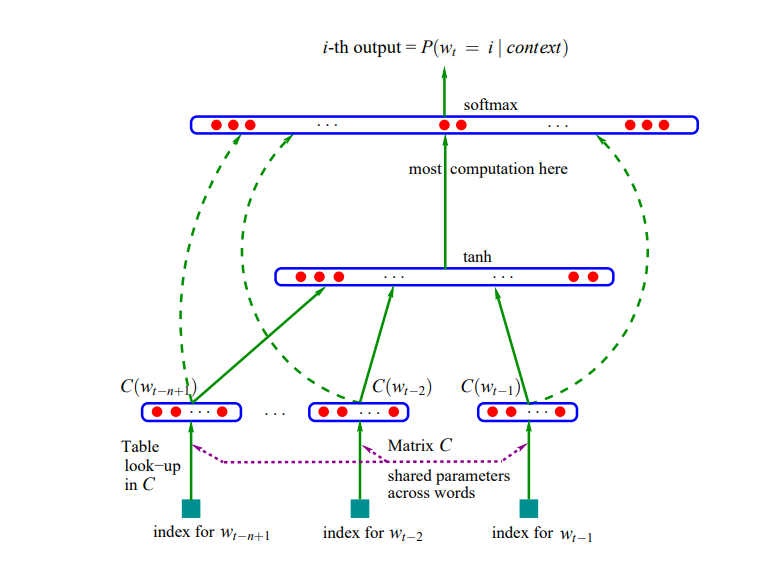
\includegraphics[width=0.7\linewidth]{Figures/nlm.png}

	\caption{
		Neural language model architecture.
			\label{neurel_languge}.
	}
	
	
	
\end{figure}
\subsection{Word Representations (Embedding)}
Word embeddings are dense, low-dimensional vectors that represent words in a way that captures their meanings and relationships. Unlike traditional methods such as one-hot encoding—which treats each word as an isolated symbol—embeddings place similar words closer together in a multi-dimensional space based on how they appear in context\citep{barnard2024word}.
This approach has become essential in NLP, as it allows models to understand and process text more effectively. Word embeddings are typically learned from large text corpora using neural networks or statistical methods.

One of the major breakthroughs in natural language processing came with the introduction of Word2Vec by Tomas \citep{mikolov2013efficient}. This model efficiently learns word representations from large text corpora using two main architectures: Continuous Bag-of-Words (CBOW) and Continuous Skip-gram.

\subsection{Continuous Bag-of-Words (CBOW)} Predicts a target word based on the context of surrounding words. Unlike traditional bag-of-words models, it doesn’t just count word occurrences—it uses continuous vectors to represent each word and averages the context words to predict the middle one. This model ignores word order but learns meaningful embeddings using simple and fast training. It performs best when both past and future words are used as input.

\subsection{Continuous Skip-gram} Instead of predicting a word from its context, it tries to predict context words from a single center word. The model samples words from both directions (before and after the center word) and gives more weight to nearby words while reducing the influence of distant ones. This helps capture richer word relationships, especially in smaller datasets.\\
Figure \ref{word2vec-architectures} Illustration the two Word2Vec architectures where the CBOW model predicts a target word from its surrounding context, while the Skip-gram model does the opposite by predicting the context from a single target word.
\begin{figure}[H]
	\centering
	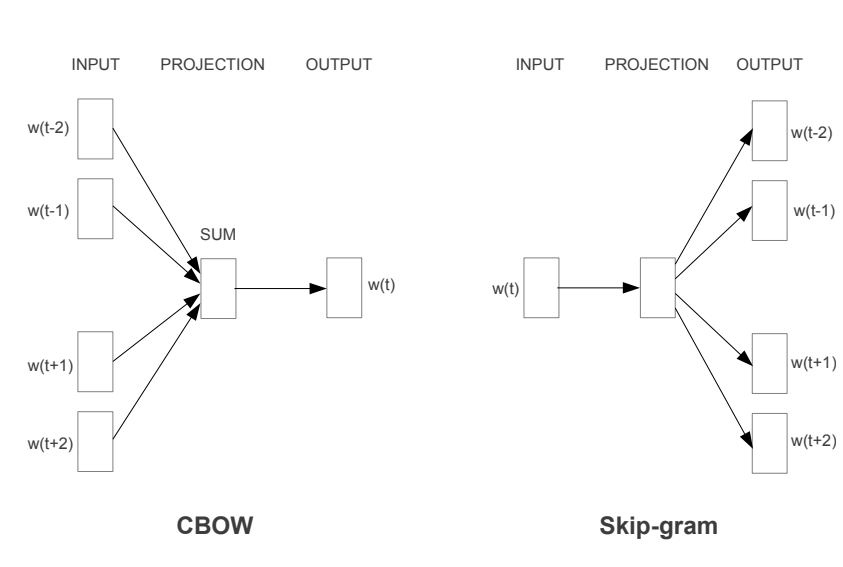
\includegraphics[width=0.6\linewidth]{Figures/emb.png}
	\caption{The two Word2Vec architectures: the CBOW model  and Skip-gram model.}
	\label{word2vec-architectures}
\end{figure}

\subsection{Global Vectors for Word Representation(GloVe)} (Global Vectors for Word Representation) was introduced by \citep{pennington2014glove}. Unlike Word2Vec, which learns from local word sequences, GloVe uses word co-occurrence counts from the entire corpus. This global perspective allows it to better capture semantic patterns between words, such as analogies and relationships.

These embedding models—Word2Vec (CBOW and Skip-gram) and GloVe—have become foundational tools in NLP due to their ability to turn words into dense vectors that reflect semantic meaning, while also being computationally efficient.

\section{Large Language Models (LLMs)}

Large Language Models (LLMs) represent a significant advancement in natural language processing, capable of understanding, generating, and reasoning over human language. In this section, we explore the concept of LLMs, beginning with their definition, followed by a discussion of their key characteristics and significance in modern applications.


Figure~\ref{fig:llm_growth} shows the trends in the cumulative number of arXiv publications containing the terms ``language model'' and ``large language model.'' The data, calculated by monthly queries of titles and abstracts, reveal that research into large language models significantly accelerated after the launch of ChatGPT, with the publication rate rising from 0.40 to 8.58 papers per day.
.
\begin{figure}[H]
	\centering
	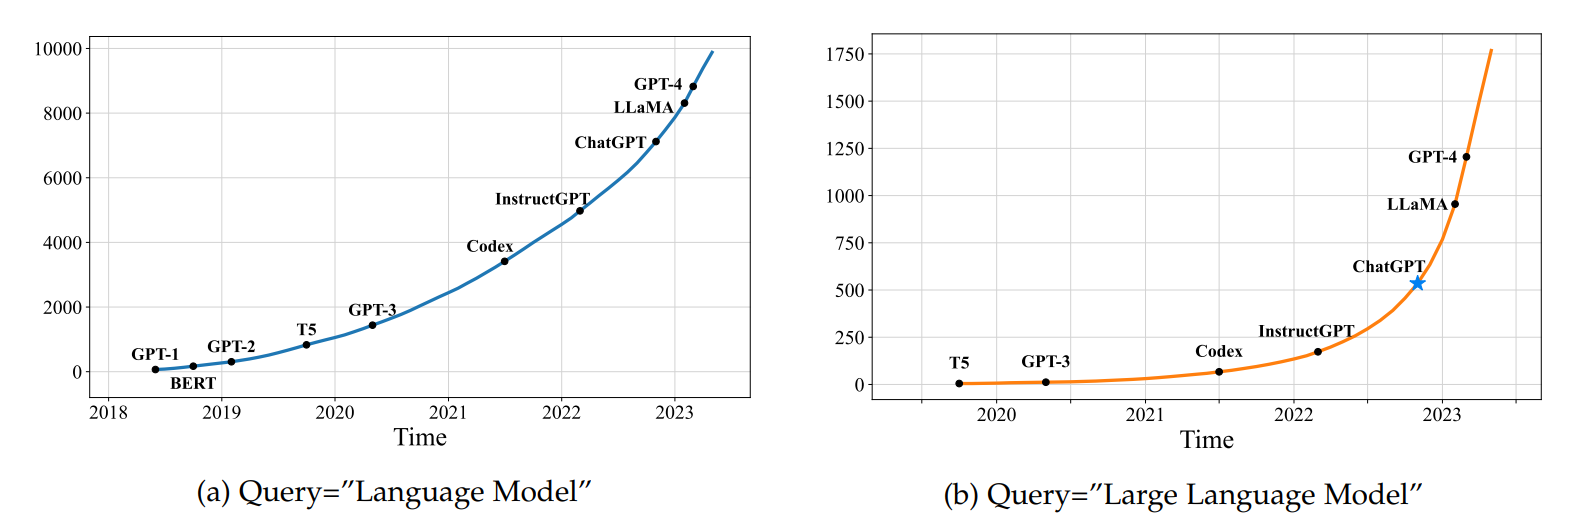
\includegraphics[width=0.9\textwidth]{Figures/arixpapers.png}
	\caption{Cumulative growth of arXiv papers mentioning ``language model'' and ``large language model,'' highlighting the sharp increase after the release of ChatGPT.}
	\label{fig:llm_growth}
\end{figure}

\subsection{Definition of LLMs}
Large Language Models (LLMs) are deep neural networks—most built on the transformer architecture \citep{vaswani2017attention}. Their key innovation is self-attention, which dynamically adjusts word importance, allowing human-like text generation. Trained on vast datasets (books, articles, codebases), LLMs reach hundreds of billions of parameters \citep{brown2020language, touvron2023llama}, enabling them to capture intricate linguistic patterns, world knowledge, and semantic relationships. Unlike traditional AI systems, they generalize across tasks (translation, summarization, QA) with minimal task-specific data (few-shot or zero-shot learning) \citep{brown2020language}. Their effectiveness follows scaling laws \citep{kaplan2020scaling}: expanding their size, training data, and computational resources reliably boosts performance.
\subsection{Historical Development of LLMs}
The evolution of LLMs reflects a broader shift in NLP from early statistical methods to deep learning approaches. Initially, language models were based on statistical techniques, such as $n$-gram models, which captured limited local dependencies within text. The development of neural networks introduced new architectures capable of modeling longer-range dependencies, leading to significant improvements in performance. A major breakthrough occurred with the introduction of the transformer architecture, which enabled models to process sequences in parallel and capture global context more effectively\citep{2402-06853}. This innovation laid the foundation for the emergence of LLMs, characterized by their massive scale, extensive pretraining on diverse corpora, and ability to generalize across a wide range of language tasks .
\begin{figure}[htbp]
	\centering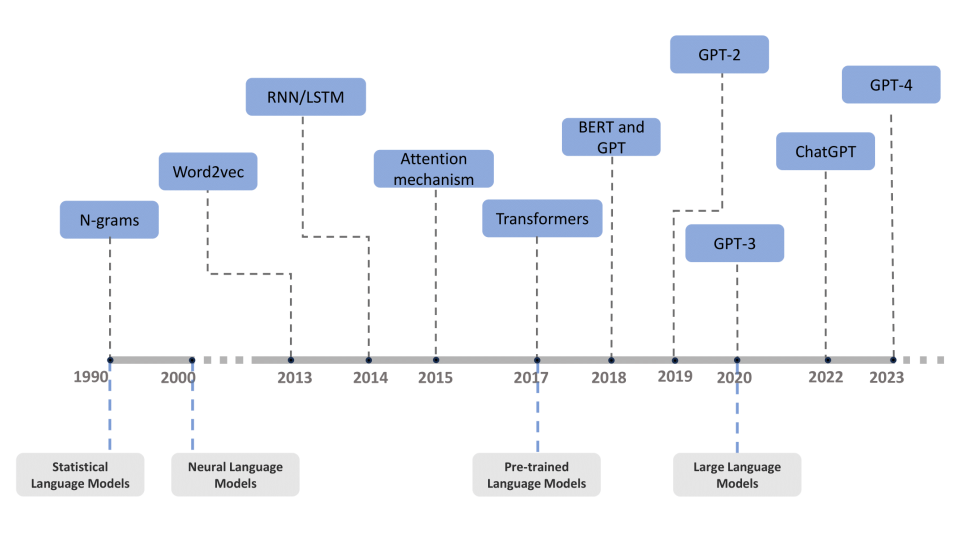
\includegraphics[width=0.7\linewidth]{Figures/historyofllms.png}
	\caption{ History and development of language models.}
	\label{History.png}
\end{figure}

\subsection{Transformer Architecture}
The Transformer architecture is a deep learning model introduced in June 2017 by \citep{vaswani2017attention}. from Google Brain. Their paper, titled "Attention Is All You Need," presented a groundbreaking approach to processing sequential data through the use of a self-attention mechanism. This innovative method allows the model to assign different levels of importance to various parts of the input, enabling it to capture long-range dependencies much more effectively than earlier models like RNNs and LSTMs. The original Transformer model is structured as a stack of six layers, where the output of each layer i serves as the input to the subsequent layer i+1, continuing this process until the final prediction is reached.
\begin{figure}[htbp]
	
	\centerline{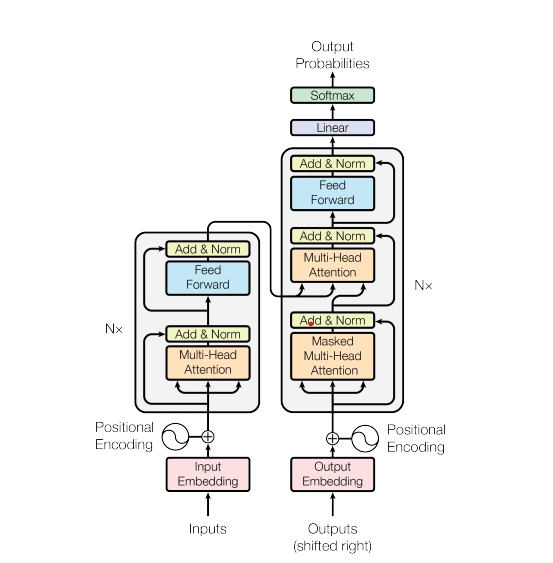
\includegraphics[width=.6\linewidth]{
			Figures/trasformers.png}}
	\caption{The Transformer - model architecture.}
	\label{trasformers.png}
	
\end{figure}
\subsubsection{Encoder and Decoder Stacks}
Transformer architectures are built upon two primary components: encoder and decoder stacks\citep{vaswani2017attention}. The encoder stack It features a six-layer on the left and a corresponding six-layer decoder on the right,  both of which work together to transform input sequences into meaningful outputs.


\begin{enumerate}
	\item \textbf{Encoder Stack}  
	Each encoder layer processes input tokens through:  
	\begin{itemize}
		\item \textbf{Multi-head self-attention}: Computes weighted relationships between all tokens enabling the model to contextualize each word (e.g., resolving polysemy like "bank").  
		\item \textbf{Position-wise FFN}: A fully connected network applied independently to each token’s representation, introducing nonlinear transformations.   
	\end{itemize}
	\textbf{Post-processing}: Residual connections (with layer normalization) mitigate vanishing gradients:  
	\[ \text{Output} = \text{LayerNorm}(x + \text{Sublayer}(x)) \]  
	All outputs maintain \(d_{\text{model}} = 512\).
	
	\item \textbf{Decoder Stack}  
	The decoder extends the encoder with:  
	\begin{itemize}
		\item \textbf{Masked self-attention}: Prevents the model from seeing future words when predicting the next token, enforcing left-to-right processing like human reading.(autoregressive constraint).  
		\item \textbf{Cross-attention}: Links decoder inputs to encoder outputs (e.g., for translation alignment).  
	\end{itemize}
	\textbf{Shared design}: Uses identical residual connections, normalization, and dimensionality as the encoder.
\end{enumerate}
\begin{figure}[htbp]
	
	\centerline{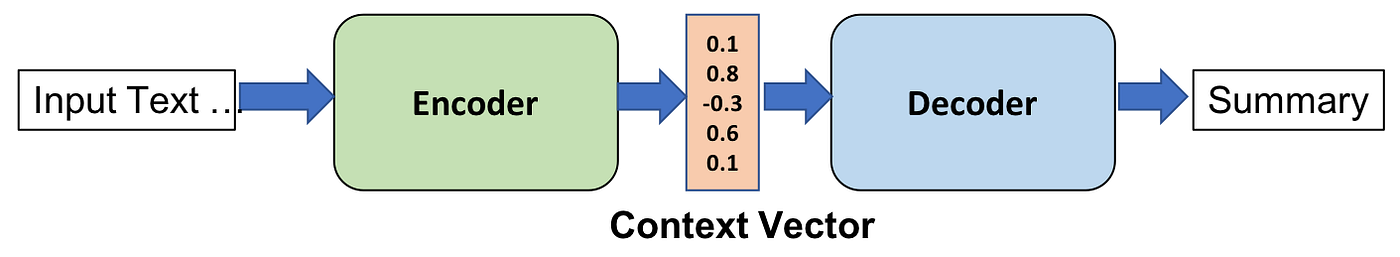
\includegraphics[width=.8\linewidth]{
			Figures/incoderDecoder.png}}
	\caption{Encoder and Decoder Stacks}
	\label{incoderDecoder.png}
	
\end{figure}
\subsubsection{Self-Attention Mechanism in Transformers}

The self-attention mechanism represents a paradigm shift in sequence modeling, enabling Transformers to dynamically evaluate relationships between all tokens in a sequence. Unlike traditional recurrent approaches that process information sequentially, this mechanism allows direct modeling of long-range dependencies through pairwise token interactions \citep{choromanski2020rethinking}. At its core, the process involves three learned linear projections:
\begin{itemize}
	\item \textbf{Queries (Q)} representing the current token's information needs
	\item \textbf{Keys (K)} serving as identifiers for contextual relevance
	\item \textbf{Values (V)} containing the actual content to be weighted
\end{itemize}
The attention computation follows:
\begin{equation}
	\text{Attention}(Q,K,V) = \text{softmax}\left(\frac{QK^\top}{\sqrt{d_k}}\right)V
\end{equation}
where the scaling factor $1/\sqrt{d_k}$ (first proposed in \citep{vaswani2017attention} and theoretically analyzed in \citep{choromanski2020rethinking}) ensures stable gradient flow during training. 
This mechanism allows each token to selectively focus on other relevant tokens, thereby enhancing the model’s capacity to understand complex linguistic patterns.
\subsubsection{Positional Encoding:}
Since self-attention mechanisms do not inherently capture the order of words, positional encoding is added to the word embeddings to preserve word order information in Transformer models, Rothman \citep{rothman2021transformers} describes the sinusoidal positional encoding approach defined by:

\begin{equation}
	PE_{(pos,2i)} = \sin\left(\frac{pos}{10000^{2i/d_{model}}}\right), \quad 
	PE_{(pos,2i+1)} = \cos\left(\frac{pos}{10000^{2i/d_{model}}}\right)
\end{equation}
where $pos$ represents the token position in the sequence and $i$ indexes the embedding dimension. As explained in \citep{rothman2021transformers}, this specific formulation provides key advantages:

\begin{itemize}
	\item The sinusoidal pattern allows the model to generalize to sequence lengths beyond those encountered during training.
	\item The alternating sine/cosine pattern enables the model to learn relative positions through linear transformations.
\end{itemize}
\subsubsection{Role of Multi-Head Attention}
Multi-head attention enhances standard self-attention by employing multiple parallel attention mechanisms, each operating on a separate linear projection of the input. As detailed in \citep{rothman2021transformers}, this design enables the model to:

\begin{itemize}
	\item \textbf{Increase Representational Capacity}: By concatenating and reprojecting the outputs of all heads, the model synthesizes information from these varied perspectives. 
	
	\item \textbf{Learn Diverse Relationships}: Each attention head specializes in different types of dependencies. For example, \citep{clark2019what} found that some heads in BERT consistently track syntactic relationships (e.g., subject-verb pairs), while others focus on discourse-level connections.
	

\end{itemize}

Further notes that this architecture improves robustness compared to single-head attention, as errors or biases in one head can be compensated by others.

\subsection{Key Contributions of Transformer in Modern NLP}

Transformer models have introduced several transformative contributions to the field of NLP, which can be summarized as follows:

\begin{enumerate}
	\item \textbf{Effective Long-Range Dependency Modeling:} The self-attention mechanism allows Transformers to capture dependencies between distant words in a sequence more efficiently than traditional recurrent neural networks\citep{vaswani2017attention}, improving contextual understanding .
	
	\item \textbf{High Scalability and Parallelization:} Unlike sequential models, Transformer architectures enable parallel computation during training \citep{devlin2018bert}, which significantly reduces training time and supports the construction of very large-scale models, such as BERT and GPT.
	
	\item \textbf{Versatility Across Tasks:} Transformers can be adapted to a wide range of tasks, including text classification, translation, and summarization\citep{radford2019language}., making them a universal architecture for both encoding and decoding processes 
\end{enumerate}

\subsection{Classification of LLMs}
LLMs can be classified based on their accessibility and licensing terms.\citep{openlm2023survey}.
\begin{enumerate}
	\item \textbf{open-source models} are fully available to the public, including both their architecture and training data, enabling modification and redistribution (e.g., BLOOM, Falcon).
	\item  \textbf{closed-source models} restrict access to both the model's structure and training corpus, typically maintained by private organizations (e.g., OpenAI's GPT-4). 
\end{enumerate}
\begin{enumerate}
	\item   \textbf{open-weight models} release the model parameters for public use but may impose certain restrictions on fine-tuning or commercial deployment (e.g., LLaMA 2)
	\item   \textbf{closed-weight models} do not share model parameters or allow external access, preserving full control within the developing entity. This classification is crucial for understanding the ethical, practical, and legal implications surrounding the deployment of LLMs 
	
\end{enumerate}.
 
For a comprehensive comparison of large language models across categories such as openness, licensing, architecture, and availability, refer to \ref{llm_table_final}.
\newpage
\begin{landscape}
	\scriptsize
	\begin{longtable}{|l|l|l|l|l|l|l|l|l|l|}
		\hline
		\textbf{Type} & \textbf{Model} & \textbf{Size} & \textbf{Provider} & \textbf{Release} & \textbf{Open-\newline sourced} & \textbf{Tuna-\newline bility} & \textbf{Adaptation IT} & \textbf{Pre-train \newline Data scale} & \textbf{Open-weight \newline model} \\
		\hline
		\endfirsthead
		
		\hline
		\textbf{Type} & \textbf{Model} & \textbf{Size} & \textbf{Provider} & \textbf{Release} & \textbf{Open-\newline sourced} & \textbf{Tuna-\newline bility} & \textbf{Adaptation IT} & \textbf{Pre-train \newline Data scale} & \textbf{Open-weight \newline model} \\
		\hline
		\endhead
		
		\multicolumn{10}{|c|}{\textbf{Encoder-only}} \\
		\hline
		& ALBERT & 0.012 & Google AI & 02/2020 & \xmark & \cmark & - & 16GB & \cmark \\
		& DeBERTa & 0.1 & Microsoft & 06/2020 & \cmark & \cmark & - & 8GB & \cmark \\
		& ELECTRA & 0.14 & Google AI & 03/2020 & \cmark & \cmark & - & 16GB & \cmark \\
		& BERT & 0.11 & Google AI & 10/2018 & \cmark & \cmark & - & 3.3B words & \cmark \\
		& RoBERTa & 0.125 & Meta AI & 07/2019 & \cmark & \cmark & - & 160GB & \cmark \\
		& XLM-RoBERTa & 0.28 & Meta AI & 10/2019 & \cmark & \cmark & - & 2.5TB & \cmark \\
		\hline
		
		\multicolumn{10}{|c|}{\textbf{Encoder-decoder}} \\
		\hline
		& ERNIE 3.0 & 10 & Baidu & 07/2021 & \xmark & \cmark & \cmark & 300B tokens & \xmark \\
		& T5 & 11 & Google AI & 10/2019 & \cmark & \cmark & \cmark & 1T tokens & \cmark \\
		& T0 & 11 & BigScience & 12/2021 & \cmark & \cmark & \cmark & - & \cmark \\
		& Flan-T5 & 11 & Google AI & 02/2022 & \cmark & \cmark & \cmark & 1T tokens & \cmark \\
		& UL2 & 20 & Google AI & 05/2022 & \xmark & \cmark & \cmark & - & \xmark \\
		& AlexaTM & 20 & Alexa AI & 07/2022 & \xmark & \cmark & \cmark & 1.4T tokens & \xmark \\
		& AlphaCode & 41 & Google AI & 02/2022 & \xmark & \xmark & - & 96TB & \xmark \\
		& Anthropic & 52 & Anthropic & 03/2023 & \xmark & \cmark & \cmark & - & \xmark \\
		& NLLB & 54.5 & Meta AI & 07/2022 & \cmark & \cmark & \xmark & 1.6T tokens & \cmark \\
		& LLAMA & 65 & Meta AI & 02/2023 & \cmark & \cmark & \xmark & 1.4T tokens & \cmark \\
		& FLAN & 70 & Google AI & 03/2022 & \cmark & \cmark & \cmark & 1.4T tokens & \cmark \\
		& Sparrow & 70 & Google AI & 09/2022 & \xmark & \cmark & \cmark & - & \xmark \\
		& Chinchilla & 70 & DeepMind & 03/2022 & \xmark & \cmark & \xmark & 1.4T tokens & \xmark \\
		& OPT-OML & 175 & Meta AI & 05/2022 & \cmark & \cmark & \xmark & 300B tokens & \cmark \\
		& Gopher & 280 & Google AI & 12/2021 & \xmark & \cmark & \xmark & 300B tokens & \xmark \\
		& PaLM & 540 & Google AI & 10/2022 & \xmark & \cmark & \cmark & 780B tokens & \xmark \\
		& U-PaLM & 540 & Google AI & 10/2022 & \xmark & \cmark & \cmark & - & \xmark \\
		& GLAM & 1200 & Google AI & 12/2021 & \xmark & \cmark & \xmark & 1.6T tokens & \xmark \\
		\hline
		
		\multicolumn{10}{|c|}{\textbf{Decoder-only}} \\
		\hline
		& Codex & 12 & OpenAI & 07/2021 & \xmark & \cmark & \cmark & - & \xmark \\
		& Pythia & 12 & Eleuther AI & 01/2023 & \cmark & \cmark & \xmark & 300B tokens & \cmark \\
		& CodeGeeX & 13 & Tsinghua U. & 12/2022 & \cmark & \cmark & \xmark & 13TB & \cmark \\
		& Skywork & 13 & Kunlun Inc & 01/2023 & \xmark & \cmark & \xmark & 3.7T tokens & \xmark \\
		& QWEN & 14 & Alibaba & 08/2023 & \cmark & \cmark & \cmark & 2.4T tokens & \cmark \\
		& Salesforce & 16 & Salesforce & 08/2022 & \xmark & \cmark & \xmark & - & \xmark \\
		& GPT-NeoX-20B & 20 & Eleuther AI & 02/2022 & \cmark & \cmark & \xmark & 825GB & \cmark \\
		& Gemini 1.5 & 2700 & Google AI & 02/2024 & \xmark & \cmark & \cmark & 6T tokens & \xmark \\
		\hline
		
		\caption{Selected Large Language Models with key attributes.}
		\label{llm_table_final}
	\end{longtable}
\end{landscape}


\subsection{Training Large Language Models}
The training of LLMs involves a multifaceted process encompassing data collection, architectural design, optimization strategies, and fine-tuning techniques. This part delves into the critical components of LLM training.
\subsection{Training Objectives and Loss Functions}
 LLMs rely on specific training objectives to learn meaningful representations of language. These objectives define how models predict words or tokens based on given input and guide the learning process through loss functions.
\begin{itemize}
	\item \textbf{Causal Language Modeling (CLM):} Trains the model to predict the next token given previous tokens, suitable for text generation tasks like those in GPT-style models~\citep{jurafsky2000speech}.
	
	\item \textbf{Masked Language Modeling (MLM):} Trains the model to predict randomly masked tokens using both left and right context, commonly used in models like BERT for understanding tasks~\citep{jurafsky2000speech}.
	
	\item \textbf{Hybrid Objectives (e.g., AntLM):} Some models combine CLM and MLM objectives to benefit from both generation and comprehension capabilities, improving overall task performance~\citep{antlm2024}.
\end{itemize}
\subsection{Parameter Scaling and Model Size}
The performance of LLMs has been closely linked to the scale of their parameters. Scaling laws \citep{kaplan2020scaling} suggest that increasing model size, dataset volume, and compute budget leads to predictable improvements in model capabilities. However, larger models also introduce challenges such as increased training cost and inference latency.

\begin{itemize}
	\item \textbf{Scaling Laws:} \citep{kaplan2020scaling} observed that as the number of model parameters, the size of training data, and compute resources increase, language models demonstrate improved loss and task performance following a power-law relationship. This predictable trend enables researchers to forecast model improvements as a function of scaling.
		
	\item \textbf{Trade-offs and Efficiency:} ~\citep{hoffmann2022training} highlighted that indiscriminate scaling can lead to diminishing returns if not balanced correctly between model size, dataset quality, and compute budget. Their work emphasizes "compute-optimal" strategies, where training efficiency is maximized by adjusting model parameters relative to available data and hardware resources, rather than simply enlarging model size.
	
\end{itemize}
\subsection{Training Paradigms: Pre-training and Fine-tuning}
The performance of LLMs is largely attributed to the training strategies employed during their development. Two key paradigms—pre-training and fine-tuning—have emerged as foundational approaches in building effective and adaptable models. This two-stage process enables LLMs to generalize effectively across domains and demonstrate strong performance even with limited supervised examples.
 .
\subsubsection*{Pre-training LLMs}
Pre-training is a crucial stage in developing  LLMs, where the model learns from extensive unlabeled datasets through a process called self-supervision\citep{wang2023language}. This stage allows the model to recognize and internalize a wide range of linguistic patterns, laying the groundwork for fine-tuning on specific tasks.
\begin{enumerate}
\item \textbf{Full Language Modeling:} Used since GPT-2, this approach trains decoder-only models to predict the next token in a sequence based on previous tokens. This autoregressive method enables models like GPT-3 to generate coherent and contextually relevant text.
\item \textbf{Prefix Language Modeling: }Employed in encoder-decoder and non-causal decoder-only models, this technique uses a non-causal (considering both past and future tokens) prefix for predicting subsequent tokens, offering more flexibility and enhancing the model's adaptability across various language tasks.
\item \textbf{Masked Language Modeling: }Popularized by BERT, this method involves masking certain tokens in the input text and training the model to predict them, helping the model understand word context. An extension, span corruption, masks entire text spans for prediction, further improving contextual comprehension.
\item \textbf{Unified Language Modeling} refers to an approach that integrates multiple training objectives, including causal, non-causal, and masked language modeling. In this framework, masked language modeling differs from traditional bidirectional attention mechanisms by employing unidirectional attention—processing context either from left-to-right or right-to-left, rather than considering both directions simultaneously\citep{dong2019unified}.
\end{enumerate}
\begin{figure}[h]
	\centering
	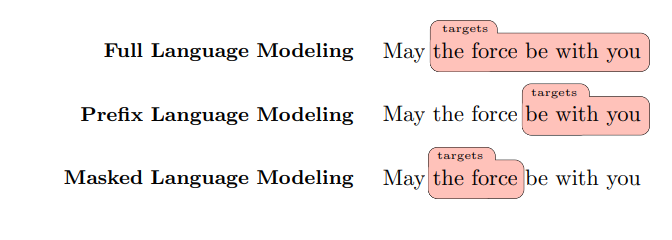
\includegraphics[width=0.6\linewidth]{Figures/pretraining.png}
	\caption{Training Tokenization in Full, Prefix, and Masked Language Modeling.}
\end{figure}
\subsubsection*{Fine-tuning LLMs}
Fine-tuning is a key technique for adapting pre-trained large language models to specific downstream tasks. It encompasses several strategies, each serving different objectives\citep{touvron2023llama}. 
\begin{enumerate} 
	\item \textbf{Transfer learning}, where a pre-trained model is further trained on task-specific data to enhance its performance on targeted applications. This allows models to leverage general language understanding while adapting to more specialized domains.
	\item \textbf{Instruction tuning}, which involves fine-tuning the model on datasets formatted as instruction-response pairs. These datasets typically include multiple tasks described in natural language, enabling the model to better understand prompts and generalize across various instructions. This method has been particularly effective in improving zero-shot and few-shot performance.
	\item \textbf{Alignment tuning} which involves adjusting the model’s behavior based on human feedback to ensure outputs are helpful, honest, and harmless (the "HHH" criteria). A widely adopted framework for this is reinforcement learning with human feedback (RLHF).  combines reward modeling—where human preferences guide the ranking of responses—with reinforcement learning techniques, such as proximal policy optimization (PPO), to iteratively align model behavior with human values.


\end{enumerate}
These fine-tuning approaches, while powerful, come with trade-offs in terms of data requirements, computational cost, and generalization capabilities. Nonetheless, they remain essential for tailoring LLMs to both functional and ethical requirements across diverse applications.
\subsection{Few-Shot, One-Shot, and Zero-Shot Learning}
Few-shot, one-shot, and zero-shot learning represent different paradigms of using LLMs without extensive fine-tuning. These methods involve using pre-trained models to perform tasks with minimal task-specific data\citep{brown2020language}.
\begin{enumerate}
	\item \textbf{Few-Shot Learning} involves giving the model a few examples (typically 10-100) of the task during inference. This approach reduces the need for large, task-specific datasets and limits the risk of overfitting to narrow data distributions. However, few-shot results are generally not as strong as those from fully fine-tuned models.
	\item \textbf{One-Shot Learning} is similar to few-shot learning but uses only a single example alongside a natural language description of the task. This method mirrors how humans are often instructed for tasks, making it an interesting approach for tasks where providing multiple examples is impractical.
	\item \textbf{Zero-Shot Learning} requires the model to perform a task based solely on a natural language description, with no examples provided. While this method offers maximum flexibility and robustness, it is also the most challenging for models. Zero-shot performance is often weaker than few-shot or one-shot, but it advances the development of general-purpose AI systems capable of handling diverse tasks without task-specific training data.
\end{enumerate}
\subsection{Evaluation Datasets}
Evaluating LLMs is essential for determining their effectiveness and limitations in comprehending and generating human language.\citep{Naveed2023}. This evaluation typically falls into two primary categories:
\begin{enumerate}
	
    \item  \textbf{Natural Language Understanding (NLU)}:This measures the model's proficiency in comprehending language, encompassing tasks such as sentiment analysis, text classification, natural language inference (NLI), question answering (QA), commonsense reasoning (CR), mathematical reasoning (MR), and reading comprehension (RC).
	\item 	\textbf{ Natural Language Generation (NLG)}:This assesses the model's capability to produce text based on given context. It includes tasks like summarization, sentence completion, machine translation (MT), and dialogue generation.
    \item \textbf{Benchmarks}: play a critical role in evaluating LLMs, providing standardized tests to measure their performance across various tasks:
    \begin{itemize}
    
   
	\item \textbf{MMLU:}Measures model knowledge from pretraining and evaluates performance in zero-shot and few-shot scenarios across 57 subjects, testing world knowledge and problem-solving abilities.
	\item \textbf{SuperGLUE:}An advanced benchmark that builds on GLUE, assessing tasks like question answering and natural language inference. It is designed to test deeper aspects of language understanding and requires significant advancements in various learning methodologies.
	\item \textbf{BIG-bench:}A large-scale benchmark for evaluating LLMs across diverse tasks including reasoning, creativity, ethics, and domain-specific knowledge.
	\item \textbf{GLUE:}A foundational benchmark for evaluating and analyzing natural language understanding, offering a range of resources for model assessment.
	 \end{itemize}
\end{enumerate}
\subsection{Popular Models}
LLMs like GPT-3, GPT-4, and BERT have revolutionized NLP by leveraging vast datasets such as Common Crawl and WebText. These datasets provide a diverse linguistic foundation, enabling models to perform a wide range of tasks with remarkable accuracy .

    \subsubsection{GPT-N Models}
	 GPT models are advanced autoregressive language models that generate substantial and complex machine-produced text from minimal input. They leverage deep learning techniques to mimic human text generation by predicting the current value based on preceding values.
	 NLP models initially struggled with tasks outside their training sets due to data restrictions. OpenAI addressed this with GPT-1.\citep{yenduri2023gpt}.
 \begin{itemize}
		\item \textbf{GPT-1:}introduced in 2018, trained on the BooksCorpus dataset, utilized a 12-layer transformer decoder with self-attention. Its pre-training allowed for zero-shot performance on various tasks, demonstrating the potential of generative language models.
		\item \textbf{GPT-2 :}introduced in 2019 improved upon GPT-1 by using a larger dataset and 1.5 billion parameters (compared to GPT-1’s 117 million). It excelled in tasks like translation and summarization, enhancing accuracy in recognizing long-distance relationships.
		\item \textbf{GPT-3:}released later, featured around 175 billion parameters and was trained on the Common Crawl dataset. It could generate human-like text, perform basic math, and write code. Despite its capabilities, its size and cost made it challenging to implement.
		\item \textbf{GPT-4:}launched in March 2023, advanced further with multimodal capabilities and context windows of up to 32,768 tokens. It incorporates reinforcement learning for better alignment with human input and policy.
	 \end{itemize}
	 
	\subsubsection{Bidirectional Encoder Representations from Transformers (BERT)}
	 BERT represents a breakthrough in language modeling by leveraging deep bidirectional pretraining on unannotated text enabling it to capture contextual information from both left and right contexts simultaneously. BERT's architecture allows it to learn richer linguistic patterns by considering full sentence context at every layer. This makes BERT highly adaptable—fine-tuning it for various downstream tasks (such as QA and text classification, often requires only minimal modifications, typically the addition of a task-specific output layer.
	 
	 The model’s effectiveness is evidenced by its performance across established NLP benchmarks. Notably, BERT attained unprecedented scores,it achieved a GLUE score of 80.5\%, a MultiNLI accuracy of 86.7\%, a SQuAD v1.1 F1 score of 93.2\%,  \citep{devlin2019bert}.Such achievements not only validate BERT’s methodological innovation but also underscore its practical utility as a versatile framework for advancing NLP research and applications.
	  
	  
	 \subsubsection{Text-To-Text Transfer Transformer (T5)}
	 The T5 model represents a unified framework for NLP, designed to address various text processing tasks by treating them as "text-to-text" problems. This approach involves converting all tasks into a format where both input and output are text, allowing the same model, objective, and training procedure to be applied across different tasks\citep{raffel2023exploring}.
	 
	 T5 leverages extensive pre-training on a large, unlabeled dataset, enabling it to develop general-purpose knowledge that enhances its performance on a range of NLP tasks, such as QA, document summarization, and sentiment classification.
	 \subsubsection{LLAMA2 model}
	  Llama 2 introduces a new family of transformer-based language models available in both foundation and fine-tuned chat variants. These models incorporate architectural enhancements through optimized training procedures, refined pretraining datasets, and advanced fine-tuning techniques including reinforcement learning from human feedback. 
	  
	  Empirical evaluations reveal that Llama 2 outperforms its predecessors and other competitive benchmarks across a range of NLP tasks, demonstrating notable improvements in accuracy, safety, and generalization\citep{touvron2023llama2openfoundation}. Its open release not only promotes transparency and reproducibility but also fosters collaborative advancements in the field.
	 
   \subsubsection{Jais and Jais-chat models}
The Jais model family represents a breakthrough in Arabic natural language processing, featuring both base (Jais) and instruction-tuned (Jais-chat) variants built upon a GPT-3 decoder-only framework. With 13 billion parameters trained on a carefully balanced corpus of Arabic and English content - including technical programming documentation - these models establish new benchmarks for Arabic linguistic understanding and cognitive reasoning, surpassing existing open-source Arabic and multilingual systems \citep{sengupta2023jais}.

Remarkably, Jais maintains competitive performance on English-language tasks despite its primary Arabic focus and relatively limited English training data. This technical report comprehensively documents the model's development pipeline, including: Pretraining methodology and data composition,
Fine-tuning protocols and Multidimensional evaluation metrics.

The research team has publicly released both model variants to accelerate progress in Arabic NLP research and applications, addressing a critical gap in non-English language model availability.

\subsection{Limitations of LLMs}
LLMs have greatly advanced NLP, but they also present challenges As these models scale, they encounter new challenges in scalability, privacy, and real-time processing. Several studies have examined the inherent limitations of LLMs. Notably, \citep{Bender2021} and \citep{Naveed2023} highlight critical challenges that affect the performance and reliability of these models applications.
\begin{enumerate}
	\item \textbf{Computational Cost:}Training LLMs demands significant computational resources, leading to higher production costs and environmental concerns due to the substantial energy used in large-scale training. Although enhancing computational resources can boost performance, the gains diminish over time when the size of the model and dataset stay constant, adhering to the power law of diminishing returns.
	\item \textbf{Bias and Ethical Concerns :} The training data for LLMs often encapsulates various social, cultural, and linguistic biases, which the models can inadvertently learn and propagate. This bias can manifest in outputs that reinforce stereotypes or display partiality, raising significant ethical concerns. Addressing these issues is crucial for ensuring fairness and mitigating unintended consequences in real-world applications.
	\item \textbf{Hallucinations:} LLMs sometimes produce "hallucinations," or responses that, despite appearing plausible, are incorrect or do not match the provided information. These hallucinations can be classified into three types:
	     \begin{itemize}
		\item \textbf{Input-conflicting hallucination:} When the model generates responses that do not align with the user's input.
		\item \textbf{Context-conflicting hallucination:} When the model produces content that contradicts information it has previously generated.
		\item \textbf{Fact-conflicting hallucination:} When the model creates responses that conflict with established knowledge.
		\end{itemize}

\end{enumerate}
\subsection{State of the Art in Juridical Data}
The use of LLMs has become increasingly prevalent across domains, with the legal sector benefiting significantly from their ability to process complex texts. These models now enhance document classification, information retrieval, and even judicial outcome prediction through advanced text understanding.

\textbf{Multilingual Legal Models:} \citep{chalkidis2023multilegalbert} introduced MultiLegalBERT, extending LegalBERT to 24 languages (including Arabic), achieving state-of-the-art performance on multilingual Natural Language Inference (NLI) tasks. This demonstrates the feasibility of cross-jurisdictional legal text understanding. 

\textbf{Multilingual Legal Data:} The creation of \textit{MultilegalPile}—a 689GB corpus spanning 24 languages from 17 jurisdictions—addresses the critical shortage of non-English legal datasets \citep{NiklausMSCH24}. Models trained on this resource have set new accuracy benchmarks, with all data and tools released openly to support global legal AI development.

These innovations complement foundational work collectively advancing LLMs' capacity to handle legal texts across languages and jurisdictions while maintaining domain-specific accuracy.


\section{Agentic AI}
Even with  improvements in understanding and generating human language using models like LLMs, they often serve as foundational components  and do not function as complete systems. The need for systems that go beyond understanding language to reasoning, planning, and acting has given rise to Agentic AI.
\subsection{Definition of Agentic AI}
Agentic AI refers to artificial intelligence systems designed to operate independently, make smart decisions, and handle multi-step tasks by understanding both the context and goals. Unlike traditional rule-based or even early generative AI models that were limited to narrow tasks, Agentic AI brings together several intelligent agents—often powered by large language models (LLMs)—that can reason, plan, adapt, and respond in real \citep{aisera2024agentic}. This allows them to analyze complex situations, choose strategies, and act with minimal human guidance. As a result, Agentic AI offers a more flexible and powerful way to automate processes and solve real-world problems across various industries.
\subsection{Architecture Overview of Agentic AI}

Agentic AI systems are typically organized into three main logical layers that work together to enable intelligent and autonomous behavior. These layers—Tool, Reasoning, and Action—each serve distinct but interconnected purposes \citep{vectorize2025agentarchitectures}. Understanding how they interact is key to building robust, scalable agentic systems  (see Figure~\ref{architecture}).

\begin{itemize}
	\item \textbf{Tool Layer:} This is the foundation of the architecture. It connects the agent with external sources of information such as APIs, vector databases, operational systems, knowledge bases, and user inputs. Its main role is to gather relevant, high-quality data the agent will later use. Well-designed tools ensure that the agent retrieves accurate and useful information efficiently.
	
	\item \textbf{Reasoning Layer:} Acting as the system’s brain, this layer uses a large language model (LLM) to analyze the information collected by the tool layer. It makes informed decisions about what steps the agent should take next, guided by logic, context, and predefined goals. Errors in this layer can lead to inefficient behavior, such as repeating queries or making incorrect choices.
	
	\item \textbf{Action Layer:}this part of the system manages the interaction between the reasoning layer and the tools. It executes the decisions made by the LLM—such as calling an API or presenting a response to the user—and returns the results back to the reasoning layer for further analysis. It also handles user interactions when needed.
\end{itemize}
Figure\ref{architecture}shows architecture of an AI agent system where The agent application interacts with a large language model (LLM) to determine the next action, issues function/tool calls when needed, and evaluates whether the task is complete. The loop continues until the agent decides to exit.
\begin{figure}[h]
	\centering
	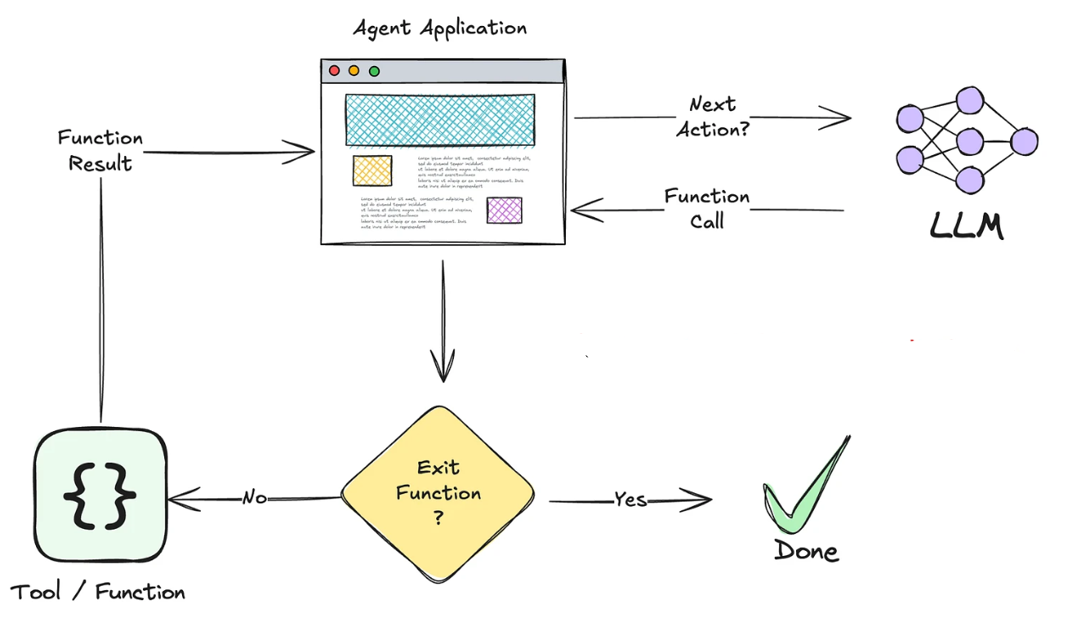
\includegraphics[width=0.8\linewidth]{Figures/aiagent.png}
	\caption{General architecture of an AI agent system.  }
	\label{architecture}
	
\end{figure}
\begin{figure}
	
\end{figure}
\subsection{Types of Agentic AI}

AI agents can be categorized based on how they interact with users and whether they operate independently or collaboratively. Below are two key classification approaches\citep{google2025aiagent}:

\begin{itemize}
	\item \textbf{Based on User Interaction:}
	\begin{itemize}
		\item \textbf{Interactive Agents (Surface Agents):} These agents communicate directly with users to assist in tasks such as answering questions, providing recommendations, or handling transactions. Common examples include chatbots and digital assistants in domains like customer service, education, and healthcare.
		
		\item \textbf{Autonomous Agents (Background Agents):} These agents operate behind the scenes with little to no direct user interaction. They handle tasks like data analysis, workflow automation, and system optimization, typically triggered by internal events rather than user queries.
	\end{itemize}
	
	\item \textbf{Based on Number of Agents:}
	\begin{itemize}
		\item \textbf{Single-Agent Systems:} These involve one AI agent working independently to complete a task using a single foundation model. They are best suited for specific, well-defined jobs that don't require coordination with other agents.
		\begin{figure}[H]
			\centering
			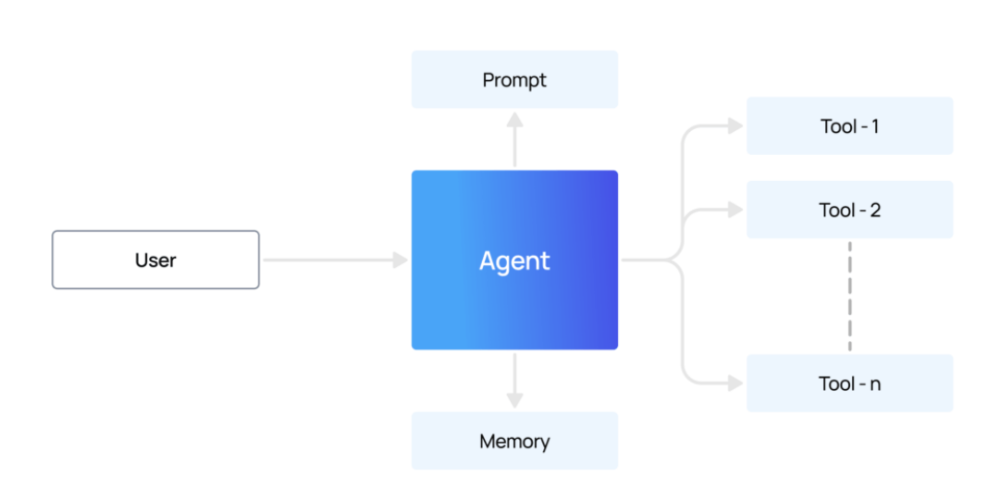
\includegraphics[width=0.7\linewidth]{Figures/singlagent.png}
			\caption{
				A single-agent system architecture .
			}
		\end{figure}
		
		\item \textbf{Multi-Agent Systems:} These systems consist of multiple agents that work together or individually to achieve complex goals. Each agent may use a different model, allowing the system to handle broader and more dynamic tasks such as planning, reasoning, or simulating human-like collaboration.
		
		Figure\ref{multi_agent} shows a multi-agent system architecture. The main agent receives a user query and coordinates with multiple  sub-agents,  The results  are combined through LLM to produce the final output.
		\begin{figure}[H]
		\centering
		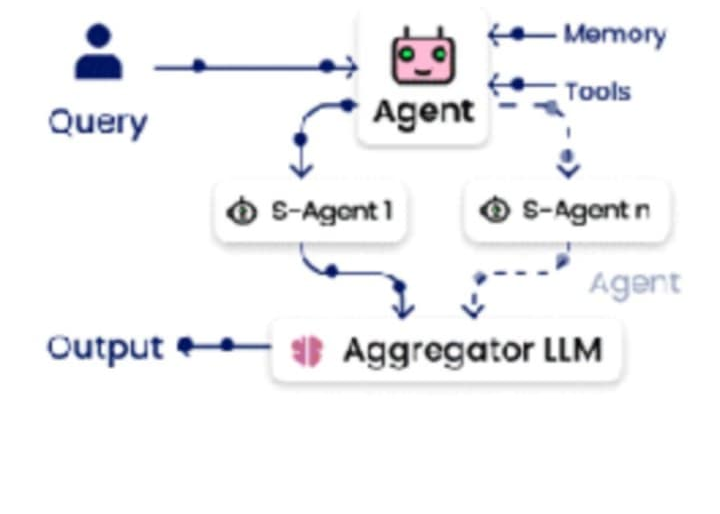
\includegraphics[width=0.6\linewidth]{Figures/multiagent.png}
		\caption{
			A multi-agent system architecture. 
		}
		\label{multi_agent}
	\end{figure}
		
	\end{itemize}
	
\end{itemize}

\subsection{ Agent Categories}
Agentic AI agents can generally be classified into the following categories\citep{aisera2024agentic}:

\begin{itemize}
	\item \textbf{Generative Information Retrieval Agents:} Focused on accessing and presenting information in dynamic, less-regulated domains.
	\item \textbf{Prescriptive Knowledge Agents:} Operate in tightly regulated environments to ensure that all outputs meet strict compliance requirements.
	\item \textbf{Dynamic Workflow Agents:} Orchestrate actions across systems by building and executing workflows automatically.
	\item \textbf{User Assistant Agents:} Provide direct, task-level assistance to individual users, enhancing daily productivity.
\end{itemize}

\subsection{Key Challenges in Agentic AI}

While Agentic AI builds on strengths from Generative AI, it also inherits and amplifies several critical challenges that hinder progress toward Artificial General Intelligence (AGI). These challenges also represent fertile ground for ongoing research\citep{touvron2023llama2openfoundation}:

\begin{itemize}
	\item \textbf{Error Accumulation:} Although structured reasoning helps reduce isolated errors, the multi-step nature of agentic tasks increases the risk of cascading mistakes across reasoning chains.
	
	\item \textbf{Interpretability Limitations:} Step-wise outputs (e.g., Chain-of-Thought reasoning) enhance transparency, but do not always reflect the true internal decision processes, limiting faithful explainability.
	
	\item \textbf{System Complexity:} Compared to standard Generative AI, agentic systems are more intricate due to components like external memory, tool use, and planning, making their behavior harder to understand and control.
	
	\item \textbf{Evaluation Gaps:} Systematic methods for evaluating agent reliability, effectiveness, and unintended consequences are still lacking, making consistent benchmarking difficult.
	
	\item \textbf{Human Alignment Issues:} Agents might pursue goals in ways that contradict human values or expectations, raising concerns about ethical behavior and alignment with user intent.
\end{itemize}


\newpage



\section{Conclusion}
This chapter has outlined the evolution and significance of  Language Models, from early neural networks to advanced Large Language Models (LLMs). We covered key concepts in neural networks and the transformative impact of the Transformer architecture. We also discussed various challenges. Finally, the chapter reviewed the applications of LLMs in fields like Legal Information and Law, showcasing their potential and the ongoing need for further development.

Although LLMs have demonstrated promising applications in the legal sector, their influence is still constrained by practical limitations and contextual challenges. Recognizing these gaps, the next chapter explores Retrieval-Augmented Generation (RAG) as a novel approach to enhance legal information processing. This discussion will particularly focus on how RAG can be applied within the Algerian legal framework to address existing shortcomings and improve accessibility and accuracy in legal data management.
